\documentclass[tikz,border=4pt]{standalone}
\usepackage{pgfplots}
\pgfplotsset{compat=1.18}
\begin{document}
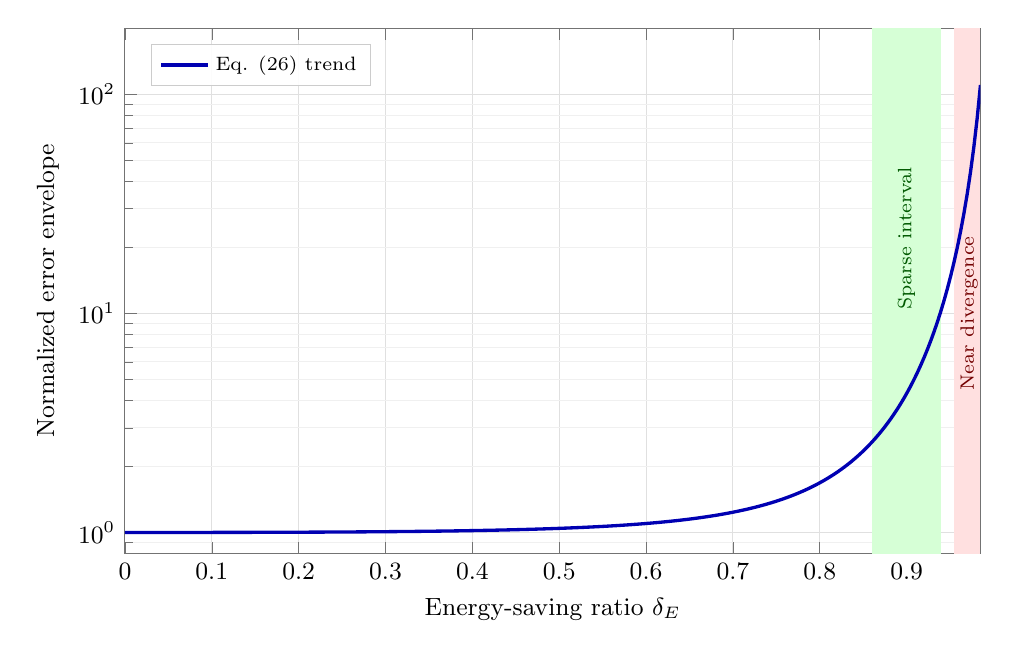
\begin{tikzpicture}
\begin{axis}[
  width=4.9in,
  height=3.25in,
  xmin=0, xmax=0.985,
  ymin=0.8, ymax=200,
  ymode=log,
  xlabel={Energy-saving ratio $\delta_E$},
  ylabel={Normalized error envelope},
  grid=both,
  major grid style={draw=black!12},
  minor grid style={draw=black!6},
  tick label style={font=\small},
  label style={font=\small},
  legend style={font=\scriptsize, draw=black!20, fill=white, fill opacity=0.92, text opacity=1},
  legend pos=north west,
  axis line style={black!55},
  tick style={black!55},
]
  \fill[green!16] (axis cs:0.86,0.8) rectangle (axis cs:0.94,200);
  \fill[red!12] (axis cs:0.955,0.8) rectangle (axis cs:0.985,200);
  \addplot[very thick, blue!70!black, domain=0:0.985, samples=260]
    {1 + 0.045*(x/(1-x+0.005))^2};
  \addlegendentry{Eq. (26) trend}
  \node[font=\scriptsize, text=green!35!black, rotate=90] at (axis cs:0.90,22)
    {Sparse interval};
  \node[font=\scriptsize, text=red!45!black, rotate=90] at (axis cs:0.972,10)
    {Near divergence};
\end{axis}
\end{tikzpicture}
\end{document}
